\chapter{Orientation Estimation}
\label{ch:orientation_estimation}

\section{Euler Angles}

Euler angles are one of several ways to describe the orientation of an object and its associated body frame in three-dimensional Euclidean space, with respect to the navigation frame, i.e. the reference frame. They represent a sequence of three elemental rotations about the axes of the coordinate system, defined as follows:

\begin{itemize}
\item The \emph{roll} angle $\phi$ determines the rotation around the $x$-axis.
\item The \emph{pitch} angle $\theta$ determines the rotation around the $y$-axis.
\item The \emph{yaw} angle $\psi$ determines the rotation around the $z$-axis.
\end{itemize}

\noindent
Figure \ref{fig:Euler_angles} depicts the rotation about the axes $z, y^{'}, Z$ by $\psi, \theta, \phi$, respectively, according to the Tait-Bryan convention. In contrast to extrinsic rotations, where the three elemental rotations may occur either about the axes of the original coordinate system, the Tait-Bryan rotations are intrinsic rotations that occur about the axes of the rotating coordinate system, which changes its orientation after each orientation. The colour blue indicates the orientation before and the colour red the orientation after the rotation.

\begin{figure}[ht]
\centering
\begin{tikzpicture}[scale=1.4]
\node[inner sep=0pt] (tait) at (0,0)
    {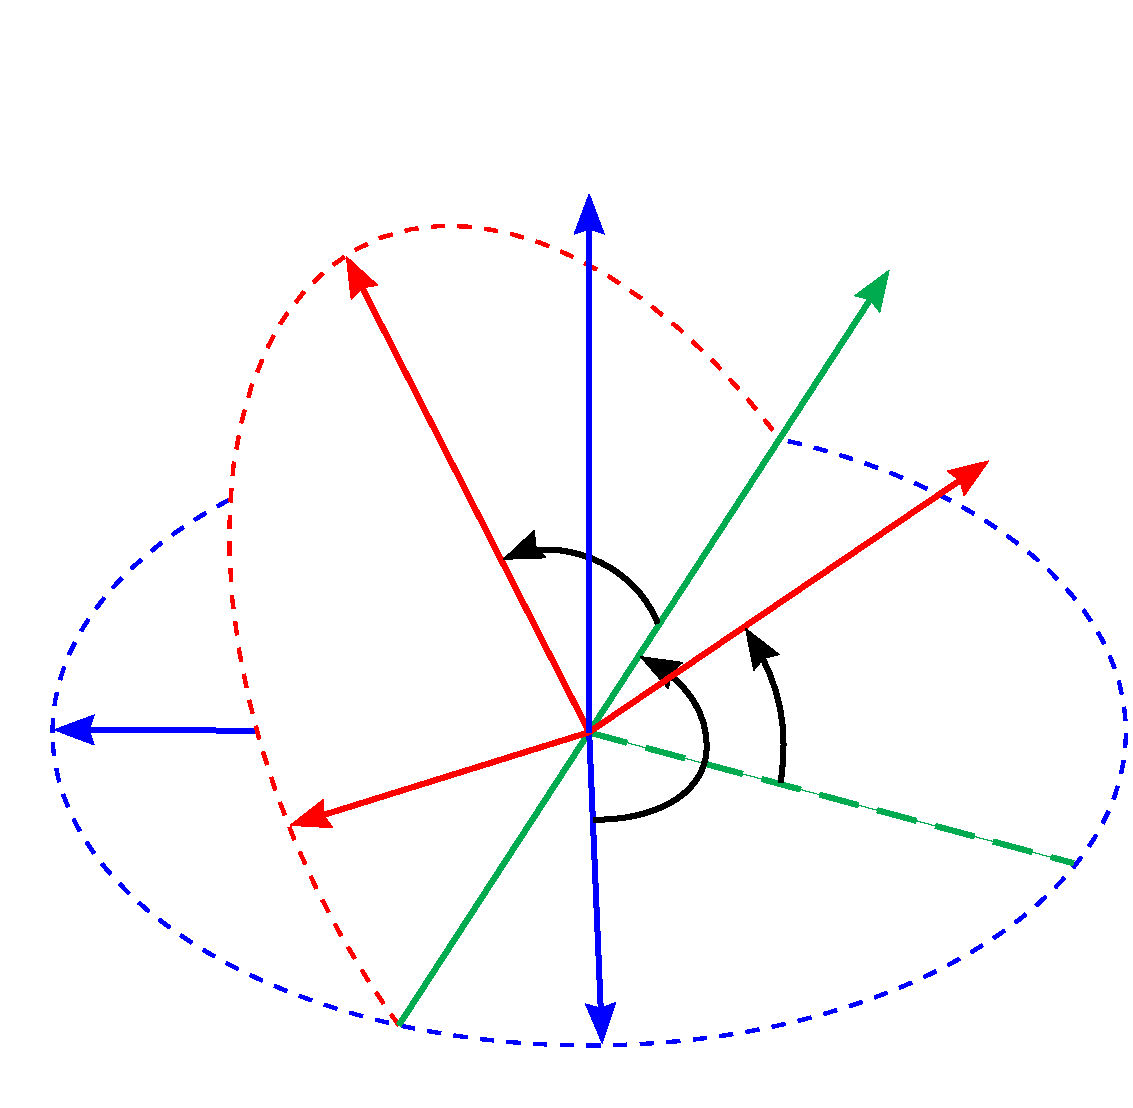
\includegraphics[width=.7\textwidth]{Images/taitbryan.pdf}};
    
\node [] at (0.5,0.2) {$\phi$};
\node [] at (0.65,-1.85) {$\psi$};
\node [] at (1.55,-0.9) {$\theta$};

\node [] at (-3.4,-1.1) {$x$};
\node [] at (0.25,-3.3) {$y$};
\node [] at (0.12,2.43) {$z$};
\node [] at (2.0,1.2) {$y^{'}$};


\node [] at (2.8,0.6) {$X$};
\node [] at (-1.5,2.05) {$Y$};
\node [] at (-2.0,-1.7) {$Z$};
\end{tikzpicture}
\caption{Representation of the body frame (red) with respect to the navigation frame (blue). The body frame was rotated, by the Euler angles $\psi, \theta, \phi$ about the axes $z, y^{'}, X$, respectively. Adapted from \cite{Wiki_taitbryan}.} \label{fig:Euler_angles}
\end{figure}

\section{Rotation Matrices}

Coordinates representing a point in one coordinate system can be transformed to another. Let $\mathbf{E}$ denote the orthonormal basis $\{x, y, z\} \in \mathbb{R}^3$ and let $\mathbf{E}^{'}$ denote the orthonormal basis $\{X, Y, Z\} \in \mathbb{R}^3$. Furthermore, let $\mathbf{b}$ be the coordinate vector of a point in three-dimensional Euclidean space. The coordinate transformation from $\mathbf{E}$ to $\mathbf{E}^{'}$ is denoted $\mathbf{\Omega}_{\mathbf{E} \rightarrow \mathbf{E}^{'}}: (b_1, b_2, b3) \mapsto (b1^{'}, b2^{'}, b3^{'})$. Then, the transformation from $\mathbf{b}$ to $\mathbf{b}^{'}$ is given by

\begin{equation}
  \mathbf{b^{'}} = \mathbf{\Omega}_{\mathbf{E} \rightarrow \mathbf{E}^{'}}(\mathbf{b}) = \mathbf{C} \mathbf{b}\,,
\end{equation}

\noindent
where $\mathbf{C}$ is the rotation matrix. To transform the coordinate vector from the navigation frame to the body frame, according to the common aerospace rotation sequence mentioned above and the Nort-East-Down system (NED), the rotation matrix $C_{nb}$ is given by

\begin{equation}
\begin{split}
\mathbf{C}_{nb} & = \mathbf{R}_x(\phi) \mathbf{R}_y(\theta) \mathbf{R}_z(\psi) \\
 & = {\left[ \begin{smallmatrix}
    1 \; & 0 \; & 0 \\
    0 \; & \cos \phi \; & \sin \phi \\
    0 \; & -\sin \phi \; & \cos \phi
    \end{smallmatrix}\right]}
    {\bigg[ \begin{smallmatrix}
    \cos \theta \; & 0 \; & -\sin \theta \\
    0 \; & 1 \; & 0 \\
    \sin \theta \; & 0 \; & \cos \theta
    \end{smallmatrix} \bigg]}
    {\left[\begin{smallmatrix}
    \cos \psi \; & \sin \psi \; & 0 \\
    -\sin \psi \; & \cos \psi \; & 0 \\
    0 \; & 0 \; & 1
    \end{smallmatrix}\right]}\\
 & = {\left[\begin{smallmatrix}
   \cos \theta \cos \psi \; &
    \cos \theta \sin \psi \; &
   -\sin \theta \\
    \sin \phi \sin \theta \cos \psi - \cos \phi \sin \psi \;\; &
    \sin \phi \sin \theta \sin \psi + \cos \phi \cos \psi \;\; &
    \sin \phi \cos \theta \\
    \cos \phi \sin \theta \cos \psi + \sin \phi \sin \psi \;\; &
    \cos \phi \sin \theta \sin \psi - \sin \phi \cos \psi \;\; &
    \cos \phi \cos \theta
  \end{smallmatrix}\right]}
\end{split}
\end{equation}

\noindent
The matrices $\mathbf{R}_y(\theta), \mathbf{R}_x(\phi), \mathbf{R}_z(\psi)$ represent the two-dimensional rotation of $\phi, \theta, \psi$ about the axes $x, y, z$, respectively. The matrix $\mathbf{C}$ is known as the Direct Cosine Matrix. Analogously, the rotation matrix $C_{bn}$ for transforming the coordinate vector from the body frame to the navigation frame is given by

\begin{equation}
\mathbf{C}_{bn} = {\left[\begin{smallmatrix}
   \cos \theta \cos \psi \; &
    \sin \phi \sin \theta \cos \psi - \cos \phi \sin \psi \; &
    \cos \phi \sin \theta \cos \psi + \sin \phi \sin \psi \\
    \cos \theta \sin \psi \;\; &
    \sin \phi \sin \theta \sin \psi + \cos \phi \cos \psi \;\; &
    \cos \phi \sin \theta \sin \psi - \sin \phi \cos \psi \\
    -\sin \theta \;\; &
    \sin \phi \cos \theta \;\; &
    \cos \phi \cos \theta
  \end{smallmatrix}\right]}
\end{equation}

\noindent
Note that $\mathbf{C}_{bn} = \mathbf{C}^T_{nb} = \mathbf{C}^{-1}_{nb}$, so that $\mathbf{C}^{ }_{bn} \mathbf{C}^T_{nb} = \mathbf{I}$.  


\section{Projection of Gravity Vector and Earth's Magnetic Field}

\section{Integration of Angular Rate}

\section{Sensor Fusion}

